\documentclass[conference]{IEEEtran}


\usepackage{cite}
\usepackage{pslatex} % -- times instead of computer modern, especially for the plain article class
\usepackage[colorlinks=false,bookmarks=false]{hyperref}
\usepackage{booktabs}
\usepackage{graphicx}
\usepackage{xcolor}
\usepackage{multirow}
\usepackage{comment}
\usepackage{listings}
%\usepackage{flushend} % even out the last page, but use only at the end when there is a bibliography
\usepackage{xspace}		% For using \SV with trailing spaces
\usepackage{cleveref}	% Needed for correctly referencing listings
\usepackage{subfig}

\newcommand{\code}[1]{{\small{\texttt{#1}}}}
\newcommand{\SV}{SystemVerilog\xspace}


% code highlighting
\usepackage{minted}
\usemintedstyle{friendly}
\setminted{fontsize=\footnotesize, frame=lines, framesep=2mm }
\newcommand\scalainline[1]{\mintinline{scala}{#1}}

% fatter TT font
\renewcommand*\ttdefault{txtt}
% another TT, suggested by Alex
% \usepackage{inconsolata}
% \usepackage[T1]{fontenc} % needed as well?

%\newcommand{\todo}[1]{{\emph{TODO: #1}}}
\newcommand{\todo}[1]{{\color{olive} TODO: #1}}
\newcommand{\martin}[1]{{\color{blue} Martin: #1}}
\newcommand{\simon}[1]{{\color{green} Simon: #1}}
\newcommand{\abcdef}[1]{{\color{red} Author2: #1}}
\newcommand{\rewrite}[1]{{\color{red} rewrite: #1}}
\newcommand{\ducky}[1]{{\color{orange} Richard: #1}}
\newcommand{\kasper}[1]{{\color{purple} Kasper: #1}}
\newcommand{\hjd}[1]{{\color{pink} Hans: #1}}

% uncomment following for final submission
%\renewcommand{\todo}[1]{}
%\renewcommand{\martin}[1]{}
%\renewcommand{\simon}[1]{}
%\renewcommand{\kasper}[1]{}
%\renewcommand{\ducky}[1]{}



%%% ZF
\usepackage{listings}
\lstset{
	columns=fullflexible,
	%        basicstyle=\ttfamily\footnotesize,
	basicstyle=\ttfamily\small,      
	%columns=fullflexible, keepspaces=true,
	numbers=left,    
	numberblanklines=false,
	captionpos=b,
	%	breaklines=true,
	escapeinside={@}{@},
	numbersep=5pt,
	language=C,
	tabsize=2,
	breakatwhitespace=true,
	breaklines=true,
	deletekeywords={for},
	%        keywordstyle=\ttfamily
	numbersep=5pt,
	xleftmargin=.10in,
	%xrightmargin=.25in
}

\newcommand{\longlist}[3]{{\lstinputlisting[float, caption={#2}, label={#3}, frame=tb, captionpos=b]{#1}}}

\title{Verification of Chisel Hardware Designs with ChiselVerify}

%\author{
%\IEEEauthorblockN{No Author Given}
%\IEEEauthorblockA{No Institute Given}
%}

\author{\IEEEauthorblockN{Order TBD before submission, Andrew Dobis\IEEEauthorrefmark{1}, Tjark Petersen\IEEEauthorrefmark{1}, Hans Jakob Damsgaard\IEEEauthorrefmark{1},\\
Kevin Laeufer\IEEEauthorrefmark{2}, Kasper Juul Hesse Rasmussen\IEEEauthorrefmark{1}, \\
Enrico Tolotto\IEEEauthorrefmark{1}, Simon Thye Andersen\IEEEauthorrefmark{1}, Richard Lin\IEEEauthorrefmark{2}, Martin Schoeberl\IEEEauthorrefmark{1}}\\
\IEEEauthorblockA{\IEEEauthorrefmark{1}\textit{Department of Applied Mathematics and Computer Science} \\
\textit{Technical University of Denmark}\\
Lyngby, Denmark \\\\
\IEEEauthorrefmark{2}\textit{Department of Electrical Engineering and Computer Sciences} \\
\textit{UC Berkeley}\\
Berkeley, CA \\\\
adobis@student.ethz.ch, s186083@student.dtu.dk, hans.damsgaard@tuni.fi, laeufer@berkeley.edu, s183735@student.dtu.dk, \\
s190057@student.dtu.dk, simon.thye@gmail.com, richard.lin@berkeley.edu, masca@dtu.dk}
}


\begin{document}

\IEEEoverridecommandlockouts
\IEEEpubid{\makebox[\columnwidth]{978-1-6654-0712-0/21/\$31.00~\copyright2021 IEEE \hfill} \hspace{\columnsep}\makebox[\columnwidth]{ }}

\maketitle

\IEEEpubidadjcol

\thispagestyle{empty}
\pagestyle{empty}

\begin{abstract}
Modern digital hardware is becoming ever more complex. The development of %Performance increase with general-purpose processors has come to a halt.
different application-specific accelerators rather than traditional %We can no longer depend on Moore's Law to increase computing performance.
general purpose processors calls for advanced development methods %The only way to achieve higher performance or lower energy consumption
not only for design, but equally so for subsequent verification. %is by building domain-specific hardware accelerators.
Recently, this has made engineers propose an agile hardware development flow. %To efficiently design and verify those domain-specific accelerators, we need
However, one of the main obstacles when proposing such a method is the lack of %agile hardware development. One of the main obstacles when proposing such a modern method
efficient tools. %is the lack of modern tools to attack it. To verify a design in such a time-constrained development
%method, one needs to have efficient tools both for design and verification.

Chisel, a high-level hardware construction language, was introduced in order to combat this lack.
Since this already enables agile hardware design, we instead focus our attention on the verification flow. %circuits described in Chisel. It builds on top of the Chisel
Thus, this paper proposes ChiselVerify, an open-source library for verifying %hardware construction language and uses Scala to drive the verification process.
circuits described in Chisel. It builds on top of Chisel and uses Scala to drive %ChiselVerify increases the productivity of the verification engineer by allowing hardware testing to be done in a modern high-level programming environment.
the verification process. The solution is well integrated into the existing Chisel 
universe, making it an extension of currently existing testing libraries.


%We implement ChiselVerify in a way inspired by the functionalities found in SystemVerilog. This allows one to use
%functional coverage, constrained-random verification, bus functional models, transaction-level modelling and much more
%during the verification process of a design in a contemporary high-level programming ecosystem.
\end{abstract}

\begin{IEEEkeywords}
digital design, verification, Chisel, Scala
\end{IEEEkeywords}

%\section{TODO}
%
%\begin{itemize}
%\item REVIEW 1: Re-write abstract and introduction - remove anything not related to verification. Remove negative wording on Verilog and VHDL. Re-consider necessity of section III.A and Fig. 2. Need for a more advanced use case.
%\item REVIEW 2: Include ChiselTest and ChiselVerify in Fig. 1. Re-write sections 4, 5 and 6, and ensure close connection to introduction. Add a few words on ChiselVerify as an agile development tool. Need for a more advanced use case (with comparison to UVM). Remove filler sentences.
%\item REVIEW 3: Prove claimed productivity increase.
%\item REVIEW 4: Need for a more advanced use case.
%\item REVIEW 5: Prove claimed productivity increase. Add table of available methods (section III).
%\end{itemize}

\section{Notes}

We will be invited to extend this paper for a journal submission. Here we start to collect ideas:

\begin{itemize}
\item Rewrite most of the text to avoid copyright issues
\item As usual, more related work \url{https://link.springer.com/chapter/10.1007/978-3-030-53288-8_19} \url{https://people.eecs.berkeley.edu/~ksen/papers/smtsampler.pdf} see also \url{https://github.com/TsaiAnson/verif/blob/master/core/src/SMTSampler.scala}
\item Comparison with UVM (performance and complexity)
\item More evaluation, e.g., use S4NOC as a non-trivial DUT
\item Use a different CSP solver
\item Kevin's formal verification work (Install Z3)
\item see also notes.tex
\item functional fuzzer
\item Use ChiselVerify/ChiselTest to test VHDL/Verilog designs
\item \url{https://docs.cocotb.org/en/stable/quickstart.html}
\item Fast test writing by using Chisel/Scala to test VHDL tests (Simon would like it)
\item Transpiling VHDL to Verilog
\item Tiling tests \url{https://github.com/TsaiAnson/verif} L2 cache \url{https://github.com/TsaiAnson/verif/blob/master/tilelink/test/TLL2CacheTest.scala}
\item \url{https://github.com/ucb-bar/riscv-mini} has bug in unaligned ld/st
\item Fuzzing paper: \url{https://compsec.snu.ac.kr/papers/hur-difuzzrtl.pdf}
\item \martin{shall bring in an arbitration circuit as a test case.} (Verification plan: a packet comes through eventually (nothing lost), no packet is ``created'' out of the air, tests under light and heavy load, measure latency and bandwidth, should be in general fair arbitration)
\end{itemize}

Some ideas from Andrew:

I think we could maybe add a part on the Queryable functional coverage and compare it to the pre-defined version. We should also completely rethink the evaluation by looking at actual performance of Chiselverify in comparison to UVM running on verilator. We could also potentially extend the constraint random stuff to add @Tjark Petersen's work but this might be a bit too much no?

We can also discuss on Slack.

\section{Introduction}
\label{sec:introduction}

\martin{rewrite}

Over the past several years, hardware design has grown to be ever more complex.
The increased demand for high-performance computing systems has lead to a larger need for domain-specific hardware accelerators~\cite{domain-hw-acc:2020}.
The design of these accelerators is often complex, and their development is time-consuming and error-prone.
In order to combat this added time-constraint, we can learn from software development trends such as agile software development~\cite{agile:manifesto}, and adapt to agile hardware development~\cite{henn-patt:turing:2019}.
Chisel~\cite{chisel:dac2012}, a Scala-embedded hardware construction language, was introduced in order to move digital circuit description to a more software-like high-level language. 

Hardware design is dominated by the traditional hardware description languages (HDLs), Verilog and VHDL, and %Many hardware engineers are switching away from the traditional hardware description %A few years ago, the two main design languages, Verilog and VHDL, dominated the
the more recent SystemVerilog. But while SystemVerilog  %languages (HDLs), i.e., VHDL and Verilog, to SystemVerilog. And while SystemVerilog %design and testing of digital circuits.
does extend Verilog with object-oriented features for verification, its hardware %%However, both languages are decades behind
description flow remains the same as with Verilog. Thus, it does not fit an agile %%modern languages for software development.
development flow. %However, compared to software development and testing, digital design and testing methods/tools 
Chisel attempts to solve these issues by providing full support for %We thus developed a method and concrete tools for agile hardware development.
functional and object-oriented programming. However, Chisel is missing efficient verification tools %ChiselVerify combines tools, languages, development, and testing methods from the last decades in
with limited functionality available in the corresponding ChiselTest package~\cite{chisel:tester2}. %software development and applies them to hardware design.

As such, we choose to base our work on Chisel and ChiselTest, and aim to raise %We developed a verification framework in Scala.
the tooling level for a digital design. We have developed a verification framework %This framework is inspired by the Universal Verification Method (UVM) but leverages Scala's conciseness with the
inspired by the Universal Verification Method (UVM), but implemented by leveraging %combination of object-oriented and functional programming.
Scala's conciseness and support for both object-oriented and functional programming. %An initial experiment of testing the accumulator circuit of the Leros processor~\cite{leros:arcs2019}
Our framework, ChiselVerify, supports both coverage-oriented and constrained %showed that a test written with UVM was about 800 lines of code, where a Scala-based
random verification (CRV) flows with more features than those available in UVM. %test was around 80 lines of code~\cite{verify:chisel:2020}.
%However, UVM supports more functionalities than a plain ChiselTest~\cite{chisel:tester2} in Scala.

As a showcase, we have verified an industrial use case, a min-heap, utilizing 
ChiselVerify to check as many features of the min-heap with as few lines of 
verification code as possible.

The main contribution of this paper is ChiselVerify~\footnote{https://github.com/chiselverify/chiselverify}, an open-source verification library for hardware designs.

The paper is organized into 6 sections.
Section II describes related work.
Section III describes background on hardware verification.
Section IV describes our solution for enabling verification in Chisel, namely ChiselVerify.
Section V explores ChiselVerify on an industry-provided use case.
Section VI concludes.

\section{The Chisel Hardware Construction Language}\label{sec:chisel}

Chisel is a modern hardware construction language embedded in the general purpose programming language Scala~\cite{bachrach2012chisel}.
It allows designers to effectively write Scala programs that generate hardware descriptions at the register transfer level (RTL).
One popular open-source application is the powerful RocketChip system on chip generator~\cite{rocketchip}.

The user-facing API of Chisel is a Scala library with some syntactic sugar that allows the user to generate RTL designs.
These designs then have to be converted into a format that is understood by simulators as well as FPGA and ASIC synthesis tools.
The lowering is done by the FIRRTL compiler which converts a high-level intermediate representation (IR) into a normalized structural representation~\cite{izraelevitz2017firrtl}.
The low-level representation is then exported into a subset of Verilog that was chosen as a common subset supported by the majority of backend tools.

Besides serving as a convenient way to lower Chisel circuits into Verilog, the FIRRTL IR and accompanying compiler infrastructure
also makes it easy to add circuit analysis and instrumentation passes.
The Chisel frontend makes it possible to attach annotations (i.e., meta-data) to arbitrary signals in the circuit and to schedule compiler passes
to be executed that are free to consume the annotations and make changes to the circuit.
We will make use of these facilities throughout the paper.



\section{Related Work}
%\todo{\url{https://capra.cs.cornell.edu/latte21/}}

\martin{rewrite}


SystemVerilog is an extension of Verilog. Many non-synthesizable extensions are intended
to write more advanced test-benches. SystemVerilog adds object-oriented programming
for those test-benches. However, in contrast to Chisel, the object-oriented addition cannot be
used for hardware description.
SystemVerilog offers certain constructs capable of gathering coverage information~\cite{spear2008systemverilog}, such as statement and functional coverage. 
When it comes to functional coverage, our solution differs in several ways from SystemVerilog. 
On top of range-based bins, ChiselVerify's \texttt{cover} constructs can take temporal relations into account, as well as generalized conditional bins that work using purely user-defined hit predicates.
This differs from SystemVerilog, which mainly focuses on bins that cover value ranges or transitions. 

The \textit{Universal Verification Methodology} (UVM) was created as a standardized way of writing test-benches on top of SystemVerilog. 
It allows for the creation of reusable test-benches (i.e., using the same test for multiple designs)~\cite{uvm2015}. 
However, it is inherently verbose, since even a simple test requires around 800 lines of SystemVerilog code. 
UVM thus requires a significant initial time-investment, but is reusable once it gets up and running. 
UVM's structure differs from most traditional test-benches, making it less accessible for newcomers than the simpler approach done by ChiselTest.

Other projects have also focused on applying software testing techniques to hardware verification. 
RFuzz~\cite{rfuzz2018} focuses on creating a generalized method that enables efficient ``coverage-guided fuzz mutational testing''. 
This method relies on FPGA-accelerated simulation and new solutions allowing for quick and deterministic memory resetting, to efficiently use fuzzing (i.e., randomized testing, where the random seeds are mutated depending on certain coverage results) on digital circuits. 
The coverage metrics used in this solution are automated and based on branch coverage. 
This work offers a different type of solution. 
While we work mostly on verification functionalities inside a language, RFuzz delivers an efficient way to use said functionalities in order to ameliorate testing. 
RFuzz uses functional coverage tools in order to guide its randomized testing. 
Current work is also being done, in the scope of the ChiselVerify project, on coverage driven mutational fuzzing for digital circuits, however this is out of the scope of this paper.


As far as we know, ChiselVerify is the only verification framework allowing for the easy use of verification functionalities, well integrated into the ChiselTest-Chisel ecosystem.

\martin{Maybe we should already reference our WOSET paper here as well: \cite{verify:fuzzing:2021}}

\martin{And somewhere also our ETS paper.}

\section{Background}
\label{sec:background}

\martin{rewrite}


This section presents a brief overview of what hardware verification is. 
We also briefly present Chisel and the current solutions that exist in it with regards to the verification of digital designs.

\subsection{Verification of Digital Designs}
Verification of digital designs refers to the testing of a design before it has been taped-out~\cite{spear2008systemverilog}. 
SystemVerilog~\cite{SystemVerilog} is one of the main languages used for verification.
The language enables verification engineers to define constraint-driven randomized test-benches and define metrics to gather functional coverage data related to a test suite. 
However, being embedded in a low-level language makes writing tests quite complex. 
The three main verification features that we are interested in are: functional coverage, constrained random verification, and bus functional modeling.

\subsubsection{Functional Coverage}
One of the main tools used in verification is test coverage. 
This allows verification engineers to measure their progress throughout the testing process and understand how effective their tests are. 
In contrast to the more common statement coverage, which defines a quantitative measure of the testing progress \textit{``How many lines of code have been tested?''}, functional coverage gives a qualitative measure, \textit{``Which functionalities have we tested?''}~\cite{spear2008systemverilog}.
Functional coverage enables the measurement of how correctly the specification has been implemented. 
This is measured relative to a verification plan, which includes the following components:

\begin{itemize}
  \item \texttt{Bin}s: Ranges of values that should be tested for (i.e., expected values of a given port).
  \item \texttt{Cover} constructs: Ports that need to be sampled in the coverage report, defined using a set of \texttt{bin}s.
\end{itemize}

\begin{figure*}
  \centering
    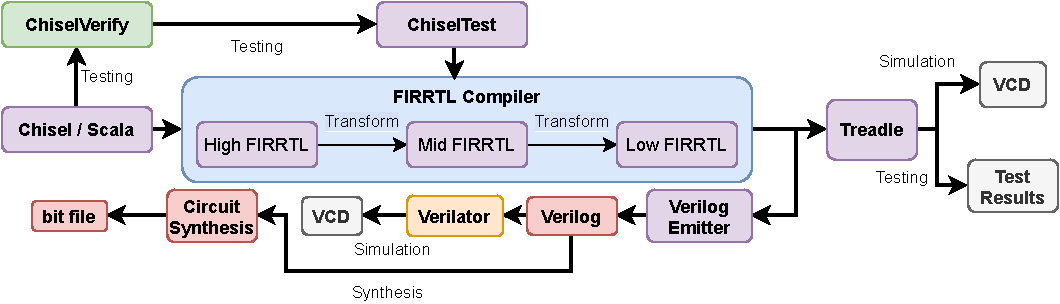
\includegraphics[width=0.8\linewidth]{Chisel_FIRRTL_VERILOG.pdf}
    \caption{Overview of the Chisel compilation pipeline. \martin{redraw}}
\label{fig:chisel-pipe}
\end{figure*}

\subsubsection{Constrained Random Verification}
CRV allows the verification engineer to create random variables which generate values that satisfy a set of associated constraints.
With constrained random inputs, a relatively small test suite can, statistically, cover many of a component's functionalities. 
In addition, the constraints help to ensure that no invalid input combinations that would not appear during regular operation are applied~\cite{MehtaCRV2018}.

These constraints define a constraint satisfaction problem (CSP).
CSP represents the entities of a problem as a finite homogeneous collection of constraints. 
CSP solvers thus serve as the basis for generating sets of constrained random signal values for verification.

SystemVerilog has native support for constrained random data types and a built-in CSP solver. 
Variables declared with the \texttt{rand} keyword are randomizable upon calling a \texttt{randomize} method.

\subsubsection{Bus Functional Models}
A bus functional model (BFM) is an abstract model of a (standardized) interface that enables interacting with manager or subordinate components at a transaction level rather than at the level of individual wires.
Many synthesis tools, including Xilinx's Vivado, provide IP generators whose output IP blocks are equipped with such interfaces. 
%Verification of components with such interfaces is most easily handled with these bus functional models (BFMs), which abstract reading and writing of signals to a transaction level. 
BFMs thus enable simpler, safer, and less verbose interactions with interfaces like, e.g., AXI.

\subsection{Digital Design with Chisel}
Our verification library is used for designs described in Chisel.
Chisel is a ``hardware construction language'' embedded in Scala, used to describe digital circuits~\cite{chisel:dac2012}.
This language is more high-level than the traditional hardware description languages, such as VHDL or Verilog, and enables object-oriented and functional programming in the context of digital design.

Since Chisel and Scala are executing on the Java virtual machine (JVM), they have an excellent interoperability with Java. 
We can therefore leverage a large pool of both Java and Scala libraries for hardware design and verification. 
Furthermore, the packaging system in Scala/Java simplifies the integration of external components.

Working in the JVM also allows for the use of the Java native interface, which enables JVM based languages to call C functions.
This enables co-simulations between Scala testers, Chisel designs, and a C-based golden model. 
This should allow companies to keep their existing C models, but move their simulation workflow into Scala/Chisel testers.

Chisel translates the hardware description into an intermediate representation called FIRRTL~\cite{firrtl}. 
It then performs multiple optimization stages, called transforms, during which high-level concepts, such as a functional map or vectors, are compiled into lower-level concepts that map onto what we usually see in a Verilog or VHDL description. 
Once that is done, the newly transformed FIRRTL, called Low FIRRTL, can be used either for simulation, using an execution engine such as Treadle, or for synthesis by translating it into Verilog, which is then used to generate the synthesized circuit. 
Note that the final Verilog description may also be used for simulation purposes using engines such as Verilator~\cite{verilator}. 
Figure~\ref{fig:chisel-pipe} shows an overview of the Chisel compilation pipeline.

\subsection{Testing Chisel Designs}
A digital design described in Chisel can be tested with ChiselTest~\cite{chisel:tester2}, a non-synthesizable testing framework for Chisel.
ChiselTest emphasizes on usability and simplicity while providing ways to scale up in complexity.
Fundamentally, ChiselTest is a Scala library that provides access into the simulator through
operations like \texttt{poke} (write value into circuit), \texttt{peek} (read value from circuit), and \texttt{step} (advance time).
As such, tests written in ChiselTest are just Scala programs, imperative code that runs one line after the next.

ChiselTest is missing fundamental verification functionalities that can improve the verification efficiency of Chisel designs. 
It is currently not possible to do things such as constrained random testing or obtaining functional coverage results while solely relying on the ChiselTest framework. 
Functionalities such as those are crucial when it comes to efficiently verify one's design.

\section{Verification with Chisel}

\martin{rewrite}


We propose ChiselVerify, a verification library written in Scala. 
ChiselVerify uses the device under test (DUT) interfacing features from ChiselTest in order to enable three main verification functionalities in Chisel: functional coverage, constrained random verification, and bus functional modelling. 
We also show how our framework can be used to create a bus functional model by creating one for the standardized AXI4 interface. 
The following subsections explain each functionality and present how to use it.

\subsection{Coverage in Chisel}
Our solution enables one to define functional coverage constructs for Chisel designs in Scala.
In order to implement the different components needed for functional coverage in Scala, we needed to be able to do the following:

\begin{itemize}
  \item Define a verification plan, using \texttt{cover} constructs.
  \item Sample DUT ports, using the ChiselTest framework.
  \item Keep track of bins to sampled value matches, using a coverage database.
  \item Compile all of the results into a comprehensible coverage report.
\end{itemize}

Implementing these elements was done using a structure based around a top-level element known as the \texttt{CoverageReporter}, enabling one to define a verification plan using a \texttt{register} method. 
This method stores \texttt{cover} construct to \texttt{bin} mappings inside a \texttt{CoverageDB} (DB being short for a database) object. 
Once the verification plan is defined, ports are sampled using the \texttt{sample} method, which is implemented using ChiselTest's peeking capabilities. 
Finally, at the end of a test suite, a functional coverage report is generated using the \texttt{report} method, which compiles the results stored in the database into a Scala \texttt{case class} which can be used to obtain coverage percentages and bin hit counts.

\begin{lstlisting}[captionpos=b,caption={Small Verification Plan defined using 3 \texttt{cover} constructs, including one cross coverage construct},label={lst:basicfuncov},language=scala]
val cr = new CoverageReporter
cr.register(
  cover("accu", dut.io.accu)(
    bin("lo10", 0 to 9),
    bin("First100", 0 to 99)),
  cover("test", dut.io.test)(
    bin("testLo10", 0 to 9)),
  cover("accuAndTest", dut.io.accu, dut.io.test)(
    cross("both1", 1 to 1, 1 to 1))
\end{lstlisting}

Listing~\ref{lst:basicfuncov} is an example of how to define a verification plan using our functional coverage tool. 
One concept used here is \textit{cross coverage} defined using a \texttt{cover} construct on multiple ports. 
Cross coverage allows one to specify coverage relations between different ports. 
This means that a cross defined between, e.g., \texttt{dut.io.a} and \texttt{dut.io.b} will be used to gather information about when \texttt{a} and \texttt{b} cover specific values simultaneously~\cite{spear2008systemverilog}.
In listing~\ref{lst:basicfuncov}, we are checking that \texttt{accu} and \texttt{test} take the value 1 at the same time.

Once our verification plan is defined, we need to decide when we want to sample our cover points using our coverage reporter.
This can be done, in our example, simply by calling \texttt{cr.sample()} when we are ready to sample our points. 
Finally once our tests are done, we can ask for a printed coverage report by calling \texttt{cr.printReport()} which results in the following: 
\begin{verbatim}
=============== COVERAGE REPORT ===============
================= GROUP ID: 1 =================
COVER_POINT PORT NAME: accu
BIN lo10 COVERING 0 to 9 HAS 8 HIT(S) = 80%
BIN First100 COVERING 0 to 99 HAS 9 HIT(S) = 9%
===============================================
COVER_POINT PORT NAME: test
BIN testLo10 COVERING 0 to 9 HAS 8 HIT(S) = 80%
===============================================
CROSS_POINT accuAndTest FOR POINTS accu AND test
BIN both1 COVERING 1 to 1 CROSS 1 to 1 HAS
1 HIT(S) = 100%
===============================================
\end{verbatim}
In the above report, we can see that our two \texttt{cover} constructs are listed and that each one of their \texttt{bins} has an associated number of hits. 
This represents how many times the port had a unique value sampled within the given range. 
A coverage percentage is then given for each bin, representing the ratio between the number of hits and the total number of possible values in the range.

Another element that our framework offers is gathering delayed coverage relationships between two coverage points. 
The idea is similar to how a \texttt{cross} works, but this time rather than sampling both points in the same cycle, we compare one port, at the starting cycle, to another port sampled a given number of cycles later. 
This number of cycles is called the \texttt{delay}, and there are currently three different ways to specify it:  
\begin{itemize}
  \item \texttt{Exactly} delay means that a hit will only be considered if the second point is sampled in its range a given number of cycles after the first point was.
  \item \texttt{Eventually} delay means that a hit will be considered if the second point is sampled in its range at any point within the following given number of cycles after the first point was.  
  \item \texttt{Always} delay means that a hit will be considered if the second point is sampled in its range during every cycle for a given number of cycles after the first point was sampled.
\end{itemize}

Finally, we exploit the functional nature of Scala in order to allow for conditional cover points, which offer the possibility to create fully custom hit-consideration rules using a user-defined predicate. 
This allows the user to check for arbitrary relations between an arbitrary number of ports. 
One could then, e.g., create a bin that considers a hit every time all fields in a vector are equal. 
This is defined simply by adding a function of type \texttt{Seq[BigInt] => Boolean} to a \texttt{cover} construct's \texttt{bin}.
The report then shows the number of hits that each condition had throughout the test suite.
Adding an ``expected number of hits'' to each condition allows for a final percentage to be shown alongside the number of hits.

These features allow for the definition of complex verification plans that can be used to represent any given specification, making it possible to verify the correct testing of any design.
In addition, supporting a coverage measure directly in the testing tool also enables modern verification strategies such as constrained random verification.

\subsection{Constrained Random Verification}

To make best use of a coverage-driven verification flow, one needs access to CRV tools. 
Such tools are, as explained before, included in SystemVerilog, and we provide another implementation in ChiselVerify. 
ChiselVerify provides a wrapper to an existing CSP solver, named JaCoP~\cite{jacop2013}, and a domain-specific language, which allows users to declare and randomize objects.

\subsubsection{Constraint Programming with ChiselVerify}
To begin writing constrained random objects using our library, one must define a \texttt{class} that extends the \texttt{RandObj} trait while initializing it with a \texttt{Model}. 
A \texttt{Model} represents a database in which all of the \texttt{RandObj}'s random variables and constraints are stored. 
This \texttt{RandObj} will then contain all of the constraints and random variables we will use in our constrained random tests. 
There are two main constructs that can be defined inside of a \texttt{RandObj}: random variables and constraints.

\paragraph{Random variables} These represent random value generators and are associated to constraints. 
Random variables can either be \textit{regular}, meaning that they can take any value satisfying the constraints, or \textit{cyclic}, meaning that they can not take the same values twice until all values have been covered.
Both types are declared using a lower and an upper bound. 
For example, if we create a \texttt{rand(0, 5, Cyclic)}, we will never get the same value twice if we sample it six times, however, on the 7th sampling, the cycle will be reset, and we will start to re-obtain old values.

\paragraph{Constraints} Constraints can either be defined alone or in \texttt{ConstraintGroup}s. 
Constraint operators are applied on random variables to create constraints.
Conditional constraints may also be defined using the \texttt{IfCond} and \texttt{ElseC} constructs. 
All of these constraints can then be enabled and disabled when needed throughout the test suite.

\paragraph{Using a RandObj} Once defined, random objects are instantiated and then randomized using the \texttt{randomize} method which returns wether or not the constraints were solvable by the CSP solver. 
The random variables can then be accessed using their respective \texttt{value()} methods.

\begin{lstlisting}[language=scala, caption={Usage of a random object. \texttt{rand(min, max, type=Normal)} is used to declare a random variable. Any operation on a random variable generates a constraint.}, label={lst:randobjscala}]    
class Packet extends RandObj(new Model(3)) {
    val idx = rand(0, 10)
    val size = rand(1, 100)
    val len = rand(1, 100)
    val payload: Array[Rand] = Array.tabulate(11)(
 	rand(1, 100)
    )

    //Example Constraint with operations
    val single: Constraint = (payload(0) == (len - size))
	
    //Example conditional constraint
    val conditional = IfCon(len == 1) {
        payload.size == 3
    } ElseC {
        payload.size == 10
    }
    val idxConst = idx < payload.size
}
\end{lstlisting}

Listing~\ref{lst:randobjscala} presents the different ways to define a random variable with constraints.
One can define collections of random variables and create constraints on those collections, as was done, for example, in the \texttt{payload} random variable. 
Conditional constraints are shown in the \texttt{conditional} random variable, where the constraint depends on the value of the \texttt{len} random variable. 

Combining constraint-random objects with the provided coverage features enables writing simple coverage-driven randomized tests. 
However, this may be further optimized by abstracting away groups of wires and operating on an operation or transaction level instead.

\subsection{Verification with Bus Functional Models}
Finally, many designers ensure portability and flexibility by equipping their designs with standardized interfaces. 
The verification engineers can test such components by combining CRV and coverage measures with BFMs to abstract their 
operation to a transaction level. In this work, we provide an example BFM for AXI4, an open standard by ARM~
\cite{axi4standard}.

\subsubsection{Introduction to AXI4}
The Advanced eXtensible Interface (AXI) protocol by ARM is a highly flexible interconnect standard based around five independent channels; three for write operations and two for read operations. Operations, known as transactions, consist of transfers across either set of channels. All channels share a common clock and active-low reset and base their transfers on ready-valid handshaking. The write channels are \textit{Write Address}, \textit{Write Data}, and \textit{Write Response}. The read channels are \textit{Read Address} and \textit{Read Data}.

Consider, for example, a write transaction of 16 data elements in which the manager first provides the transaction attributes (e.g., target address and data size) as a single transfer over the \textit{Write Address} channel followed by the 16 data elements one at a time over the \textit{Write Data} channel. Finally, the subordinate indicates the status of the transaction over the \textit{Write Response} channel. Beware that the write data may be transferred prior to the transaction attributes due to channel independence, and similarly, the \textit{Read Address} and \textit{Read Data} channels may operate independently at the same time~\cite{axi4standard}.

\subsubsection{Implementation}
Our implementation of an AXI4 BFM includes bundles defining the five different channels, abstract classes representing both manager and subordinate entities, transaction-related classes, and the BFM itself, the \texttt{FunctionalManager} class. The BFM is parameterized with a DUT that extends a \texttt{Subordinate} class and provides a simple, transaction-level interface to control the DUT. As such, its two most important public methods are \texttt{createWriteTrx} and \texttt{createReadTrx}, which do precisely as their names indicate; create and enqueue write and read transactions.

Internally, the BFM makes use of ChiselTest's multithreading features to allow for (a) non-blocking calls to the methods mentioned above (i.e., one can enqueue multiple transactions without waiting for their completion) and (b) emulating the channel independence more closely. When, for example, a write transaction is enqueued, and no other write transactions are in-flight, the BFM spawns three new threads, one for each required channel. The threads each handle the handshaking necessary to operate the channels.

\subsubsection{A Test Example}
Consider as an example using the BFM to test a module called \texttt{Memory}, as shown below. Creating a write transaction with 16 data elements (minimum burst length is 1, hence \texttt{len = 15} means a burst of 16 items) takes just one call to a method the majority of whose arguments have default values. It is equally simple to create a subsequent read transaction. Beware that due to channel independence, not waiting for a write to complete before starting to read from the same address may return incorrect results depending on the implementation of the DUT.
\begin{lstlisting}[language=scala, caption={Using the AXI4 BFM with ChiselTest}, label={lst:axitest}]
class MemoryTester extends FlatSpec with ChiselScalatestTester {
  behavior of "My Memory module"
  it should "write and read" in {
    test(new Memory()) { dut =>
      val bfm = new FunctionalManager(dut)
      bfm.createWriteTrx(0, Seq.fill(16)
      	(0x7FFFFFFF), len = 15, size = 2)
      bfm.createReadTrx(0, len = 15, size = 2)
    }
  }
}
\end{lstlisting}

\section{Formal Verification}

% introduce dynamic verification
% While working on the RTL level description of a new circuit, designers need to quickly test their design
% in order to iteratively improve it. Extensive testing is also a common requirement before sending a design to be
% fabricated as bugs discovered after ASIC fabrication can be costly or even impossible to fix.
% The most common approach to testing RTL is to write a test bench program that interacts with a simulation of the design.
% Errors are found through manual waveform inspection or assertions in the design or the test bench.

% explain bounded model checking
An alternative to exercising the circuit description with a set of concrete inputs is to symbolically explore the circuit execution
for any inputs for a limited number of cycles.
This technique is called bounded model checking~\cite{bmc} and works by unrolling the circuit for $k$ cycles and then asking a
SAT~\cite{sat} or SMT~\cite{smt} solver whether there exists a set of inputs and starting states for the memories and registers in the
design, for which an assertion is violated.
If the solver returns a satisfying assignment to this query, we obtain a counter example that can be expressed as a test bench that
initialized the state to concrete values from the solver and then drives the inputs for $k$ cycles with the inputs obtained from the solver.
If the solver returns that there is no such assignment, we get a guarantee that our circuit will not hit any assertion violation for the first $k$
cycles of its execution.

\begin{figure}
    \centering
\begin{minted}[
fontsize=\footnotesize,
frame=lines,
framesep=2mm,
]{scala}
class Quiz15 extends Module {
  /* [...] I/O definitions */
  val mem = SyncReadMem(256, UInt(32.W), WriteFirst)
  when(iWrite) { mem.write(iWAddr, iData) }
  oData := mem.read(iRAddr, iRead)

  when(past(iWrite && iRead &&
            iWAddr === iRAddr)) {
    verification.assert(oData === past(iData))
  }
}

class ZipCpuQuizzes extends AnyFlatSpec
  with ChiselScalatestTester with Formal {
  "Quiz15" should "pass with WriteFirst" in {
    verify(new Quiz15, Seq(BoundedCheck(5)))
  }
}
\end{minted}
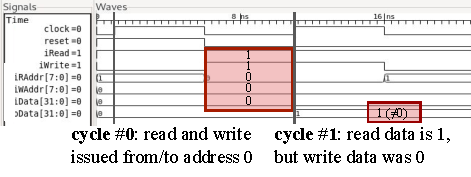
\includegraphics{woset_2021_quiz15.pdf}
\caption[Chisel verification example.]{This example verifies that when a Chisel memory with synchronous read port and
\scalainline{WriteFirst} behavior has a read and a write access to the same address,
the new value will be returned.
The check fails if \scalainline{WriteFirst} is substituted with \scalainline{ReadFirst} or \scalainline{Undefined} (Section~\ref{sec:undef}).
It is based on \href{https://zipcpu.com/answer/2021/07/03/fv-answer15.html}{a Verilog example from a popular blog}.
In the Chisel version, the assertion is automatically delayed until at least one cycle after reset, when there are valid \scalainline{past} values available
(Section~\ref{sec:past}).
A bounded model check is executed by the \scalainline{verify} command, which is called from a standard Scala unit test (Section~\ref{sec:flow}).
When the check fails, the failing inputs and starting states are replayed on a simulator, resulting in a waveform file that is identical
to the output we would get from a dynamic verification run.
However, since we used bounded model checking to find the failing trace, it will be as short as possible.
In our example, two cycles after reset are needed to fail the property.
The first cycle contains the read and write requests and the second cycle observes the arbitrary result on the read port if
we set the memory behavior to \scalainline{Undefined} for read/write conflicts.
The included screenshot was obtained with the open-source GTKWave waveform viewer.
}
\label{fig:quiz15}
\end{figure}

% the current state of the open-source ecosystem for formal verification
There has been a long tradition of open-source formal verification systems from the academic community~\cite{mcmillan1993smv, cimatti2000nusmv, mishchenko2007abc}.
% only citing select solvers for space gains
%~\cite{mann2021pono, mcmillan1993smv, cimatti2000nusmv, owre1996pvs, goel2020avr, vizel2014interpolating, mishchenko2007abc}.
However, because of the traditional academic incentive structure, these research systems were hard to use or did not support
enough features of the RTL design language to be widely used by a community of open source RTL designers.
This changed with the introduction of the yosys~\cite{yosys} tool which has become the de facto standard for processing
Verilog for synthesis or formal verification.
Yosys allows academics to focus on developing model checkers for the simple btor2~\cite{btor2} or aiger~\cite{aiger} formats
without having to worry about supporting the much more complicated Verilog standard.
The open-source SymbiYosys~\cite{symbiyosys} tool wraps yosys as well as various formal verification engines in order to allow users to
verify their designs. All a user has to provide are the Verilog sources of their design including assertions and assumptions
as well as a small configuration script. SymbiYosys translates any failing traces it discovers into Verilog test benches and VCD waveform dumps
for the user to inspect~\footnote{With the open-source GHDL plugin, yosys now also supports formally verifying VHDL circuits.}.


% problems with the SymbiYosys approach
In this paper we describe our approach to providing Chisel users with an easy way to formally verify their designs.
We adapt many good ideas from yosys and build several new convenience features on top of them, taking advantage
of the existing compiler infrastructure for Chisel.

\subsection{Our Formal Verification Flow}\label{sec:flow}


Before we dive into some of the details of our implementation we want to present
the workflow that we imagine and illustrate how easy it can be to get started
with formal verification of a Chisel circuit~\footnote{
A scala project with executable examples as well as a Jupyter notebook are included in the companion repository to this paper:
\url{https://github.com/ekiwi/open-source-formal-verification-for-chisel}.
The contributions described in this paper are all part of the upstream \href{https://github.com/chipsalliance/firrtl}{firrtl}
and \href{https://github.com/ucb-bar/chisel-testers2}{chiseltest} libraries.
}.
The recommended way to start a Chisel project is to use the open-source Chisel template 
repository~\footnote{\url{https://github.com/freechipsproject/chisel-template}}.
The resulting Scala project automatically includes dependencies on the Chisel and the chiseltest
libraries which will be downloaded by the Scala build tool.

The template contains an example of using the chiseltest library to test a greatest common denominator (GCD) circuit in simulation.
This test can be executed through a Scala IDE or from a shell with the \scalainline{sbt test} command.
In order to turn this test into a formal check, we just need to substitute the \scalainline{test(new DecoupledGcd(16))}
command with \scalainline{verify(new DecoupledGcd(16),} as well as provide the type of verification job as
\scalainline{BoundedCheck(10)} and extend the testing class with the \scalainline{Formal} trait.
If the user now clicks the test icon again or runs the \scalainline{sbt test} command, a formal bounded check will
be executed for ten cycles after reset instead of a simulation test.
The only additional program required is a copy of the open-source SMT solver Z3~\cite{de2008z3}.



\begin{figure}
\centering
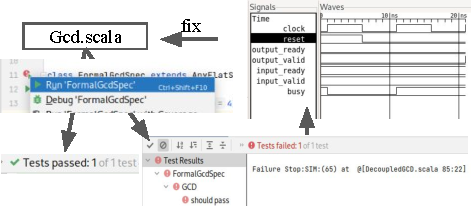
\includegraphics{woset_formal_ide_flow.pdf}
\caption{When working in a standard Scala IDE like the open-source IntelliJ IDEA with the Scala plugin, the user can launch the formal check with the press of a button.
The success or failure will be communicated the same way as any other unit test. A VCD waveform dump is automatically generated to help debug failing checks.}
\label{fig:ide-flow}
\end{figure}

Initially the check will always pass, no matter which changes we make to our circuit.
Since the GCD circuit contains no assertions, there is nothing to tell the solver if the circuits misbehaves.
In order to actually verify something, we can add assertions directly to the circuit by using the
Chisel \scalainline{assert} statement.
The decoupled GCD circuit used as an example has an \scalainline{input} and an \scalainline{output} channel
as well as a 1-bit \scalainline{busy} register.
We expect that while the circuit is busy, no new input is accepted:
\begin{minted}{scala}
when(busy) {
  verification.assert(!input.fire())
}
\end{minted}
This assertion will pass because the circuit does indeed fulfil the property after reset.


We now introduce a small bug by connecting \scalainline{input.ready} to \scalainline{true.B} and rerun the test
An assertion violation will be reported one cycle after reset.
The user is also presented with an error message indicating the Scala line number of the failing assertion.
To debug the problem, they can find a VCD waveform dump in the standard test directory created by our
chiseltest library.
Since we replay the test on a concrete simulator, the error message and VCD will be exactly the same
as if the user was running a simulation test.
% Any improvements to our simulation interface or error reporting will thus immediately benefit formal verification
% users as well.

A more advanced property we expect to hold is that if the input and output channels are idle, the busy
signal will remain the same in the next cycle:
\begin{minted}{scala}
when(past(!input.fire() && !output.fire())) {
  verification.assert(stable(busy))
}
\end{minted}
Here we make use of our \scalainline{past} function for temporal properties which is described in detail in Section~\ref{sec:past}.



\subsection{A Formal Backend for FIRRTL}\label{sec:undef}

\begin{figure}
\centering
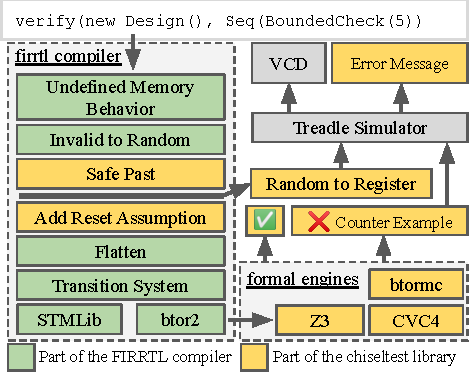
\includegraphics{woset_verify_flow.pdf}
\caption{The \scalainline{verify} command is implemented as part of the chiseltest library and uses several compiler passes that make up the FIRRTL formal backend.
We hook into the FIRRTL compiler to model undefined behavior with \scalainline{DefRandom} statements and to delay temporal assertions as part of our safe past construct.
We then add reset assumptions, flatten the system, convert to a formal transition system and then serialize the system to SMTLib or btor2.
We provide bindings to launch various formal engines from chiseltest.
If a counter example is found, we convert the \scalainline{DefRandom} nodes in the circuit to registers before loading the circuit into the treadle simulator
to replay the failure and obtain a simulation quality VCD and error message.}
\label{fig:verify-flow}
\end{figure}

In order to implement the verify command introduced in the previous section, we need to convert the Chisel circuit into a format that is understood
by open-source model checkers or SMT solvers.
We can do this by using the FIRRTL compiler to convert the circuit to Verilog and then using yosys to convert to the
model checking formats.
While we initially used this approach, we eventually decided that it would be better to add a formal backend to the FIRRTL
compiler directly.
This way we can avoid the complicated Verilog semantics, model circuit behavior in greater detail and easily replay counter
example traces on our FIRRTL simulator called treadle.

Users want their Chisel designs to be implemented with as little hardware as possible.
In order to allow for efficient implementations, the FIRRTL specification was crafted to allow
some operations to result in arbitrary results.
For example, a wire connected to \scalainline{DontCare} or to the result of a division by zero carries an arbitrary value.
Reading from a memory while the read port is disabled, reading from the same address that another port is writing to or
writing from two memory ports to the same address all generate an arbitrary value result.
Not all of these behaviors are represented in the generated Verilog.
The compiler is free to substitute arbitrary with (more) concrete values, like always returning a memory read result even
when the read port is disabled or by assigning a priority to write operations so that at least one of them will complete.
Thus if we first generate Verilog and then use yosys, we are only verifying one concrete translation of the design,
but there may be other legal translations that would violate the property.
This is relevant, e.g., in the context of memories when we use an external SRAM compiler that might try to
rely on the fact that write-write collisions can have arbitrary results in order to generate better hardware.
This is the reason why we decided to carefully model arbitrary values as part of the FIRRTL compiler's new formal backend.

Once the formal engine finds starting states and inputs that lead to an assertion violation, we need to help the user debug their design.
Since we do not have the large resources of a major EDA vendor, we would like to reuse as much of the existing simulator infrastructure as we can.
If we can replay the failing trace on our existing simulator, the VCD waveform dump and the error reporting will be of the same quality as
when writing a concrete test bench.
In order to be able to replay failures caused by arbitrary values, we carefully engineered two FIRRTL passes that analyze the circuit and
add wires to detect when a result is arbitrary as well as a mux to substitute the result with a connection to a \scalainline{DefRandom} node in that case.
The new \scalainline{DefRandom} construct provides a named arbitrary value which can change every clock cycle,
very much like a \scalainline{anyseq} annotated wire in Verilog.
The formal backend implements \scalainline{DefRandom} nodes as inputs that can be freely chosen by the formal engine.
To make \scalainline{DefRandom} work with our simulator we  replace the nodes with registers of the same type that are never updated by the hardware.
Instead we use the software interface to our simulator to update these registers with the values chosen by the formal engine in each cycle.
Figure~\ref{fig:verify-flow} shows our compilation flow in more detail.

The btor2 format does not support hierarchical circuits and we thus always flatten the system by inlining everything into a single module.
In order to ensure that we produce a good waveform dump, the counter example will be replayed on the non-inlined circuit.
We make use of the built-in annotation support of the FIRRTL compiler to automatically track name changes of all registers and memories in
the design as they are inlined. This way we can map initial states found by the formal engine back to their hierarchical names.

Once the circuit has been flattened, the conversion to a transition system is fairly straight forward.
We implemented a SMTLib and btor2 encoding that is very similar to the one pioneered by yosys.
We used the FIRRTL specification to accurately translate FIRRTL expressions to the bit-vector expression language defined by the SMTLib format~\cite{smtlib}.
Our backend supports memory and register initialization using the same user annotations as the Verilog backend.
Multi-clock support through a clock stuttering pass is work in progress, for now only circuits with a single clock domain are officially supported.

\begin{figure}[t]
  \centering
  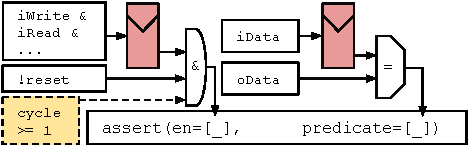
\includegraphics{woset_safe_past.pdf}
  \caption{The temporal assertion from Figure~\ref{fig:quiz15} results in a circuit with two registers created by the \scalainline{past} function:
  One to delay the condition from the \scalainline{when} statement and the other to delay the input data before it is compared to the current output data.
  By default an assertion is only enabled when reset is inactive and the surrounding \scalainline{when} condition is true.
  Our compiler pass analyzes the connectivity graph with the result that both the enable condition as well as the predicate are delayed by a single past register.
  Thus the assertion enable signal is automatically extended to include the condition that at least 1 cycle must have past since the last reset.
  The new enable condition is derived from a synthesizable, saturating \scalainline{cycle} counter which is created by the compiler pass.
  }
  \label{fig:past}
  \end{figure}
  

\subsection{Reset Assumptions}\label{sec:reset}

In Chisel, users rarely need to worry about resets.
Registers with reset values are automatically connected to the default reset % port of the module
and module instances just inherit their reset domain from their parent.
In Verilog, users have to manually ensure that assertions are only triggered after the circuit was properly reset.
We decided to provide sensible defaults instead.
Assertion statements are automatically disabled, just like it has been the case for print and stop statements
since the early days of Chisel.
As part of our formal verification support, we provide a FIRRTL pass
that automatically adds a constraint for the reset of the top level module to be active during the first cycle of execution.
Thus, by default, users do not have to worry about reset. Their assumptions will only fire
after their circuit has been properly reset and hence we ensure that there are no false positives.
We do provide options for power-users to write assertions that are active during reset and to
disable reset assumptions or increase the number of reset cycles.


\subsection{Simple Temporal Assertions}\label{sec:past}


While a simple \scalainline{assert} statement allows us to specify a property over signals during a single
cycle, it is not enough to express properties that require us to reason about multiple cycles.
The traditional answer to this problem are temporal assertion languages like SystemVerilog Assertions~\cite{SystemVerilog}.
However, these are complex to implement efficiently and as of now there has not been a successful open-source implementation.
The community around SymbiYosys has instead advocated for the use of plain assertions with the Verilog \scalainline{past}
function. This function returns the previous value of an expression and thus allows us to write properties that span multiple cycles.

While conceptually simple, the \scalainline{past} construct as defined by the Verlog standard has one major problem:
In the first cycle of the circuit execution, there is no past value and the \scalainline{past} function always returns X.
Thus the user has to take care to keep track of how many cycles have past since the verification started and only enable assertions
once all past values are valid.
This particular pitfall is often the topic of a \href{http://zipcpu.com/quiz/2019/11/16/quiz07.html}{popular formal verification quiz}.
%In addition to that, \scalainline{past} values can also be invalid because they happened while
%the circuit was going through reset.

We made use of some of the unique capabilities offered by Chisel in order to implement what we consider to be a safer version of the
\scalainline{past} function.
In the frontend, our \scalainline{past} is a Scala function which creates an appropriate amount of delay registers in the current
clock and reset domain. That alone provides functionality similar to the Verilog version of \scalainline{past}.
We go further by annotating the delay register and asking for a FIRRTL pass to be run when lowering the design.
This pass looks at a graph of all \scalainline{past} delay registers and assertions in a module.
An edge indicates that the input to the assertion or register is connected to the output if a delay register through combinatorial logic.
We traverse the resulting tree (by design there can be no cycles) starting at each assertion
to find the longest path of \scalainline{past} delay registers in order to determine the number of cycles the assertion needs to be delayed.
Finally we generate a cycle counter register and use its value to guard the individual assertions.
Since our \scalainline{past} function only relies on synthesizable hardware it can also be used in software and FPGA based
simulation testing~\cite{karandikar2018firesim}.






\section{Evaluation}

We evaluate our ChiselVerify with two application examples. \todo{continue to write}

\subsection{An Arbitration Circuit}

We evaluate ChiselVerify with an arbiter circuit. The arbiter uses a ready/valid interface for the clients
and the shared resource. The arbiter is build as a binary tree, where each node does a local arbitration
and contains a register to store the data until it can be communicated further up towards the root of the
tree. Each local 2 to 1 arbiter has turn flag to be fair between the two requests. The assumption is that
this local fairness translates to a global fairness of the full arbitration tree.

To test the arbiter, we specify properties that result in a verification plan:

\begin{itemize}
\item Each request shall eventually be seen at the output (the root node)
\item Now requests shall be ``generated'' in the tree (out of thin air)
\item The maximum latency for a request shall be $n$ cycles without any competing requests
\item The maximum latency for a request shall be $m$ cycles under full load
\item The arbitration shall be fair, which means the bandwidth difference between clients shall be bound by $x$ \%.
\end{itemize}

The values of $n$, $m$, and $x$, depend on the number of clients, i.e., the size of the arbitration
circuit.

\martin{Show that the Chisel treeReduce is broken and show our solution. Need to copy that test
over. And we provided as a solution a PR for Chisel \url{https://github.com/chipsalliance/chisel3/pull/2318}}



\subsection{Sorting in Hardware}

\martin{rewrite}


In our research, we received a use case from Microchip~\cite{microchip} in the form of a specification.
We implemented and used it to evaluate our verification library.

\subsubsection{Specification}

The provided use case is a hardware implementation of a priority queue, which can be used in real-time systems requiring scheduling capabilities. 
For instance, timestamps for deadlines can be inserted and sorted such that the host system has access to the closest deadline.

Internally, the hardware priority queue relies on a min-heap tree data structure. 
The run-times of insertion and removal operations, both having a complexity of $O(\log_k N)$ where $N$ is the number of elements and $k$ the number children per node, are bound by the depth of the tree. 
By increasing $k$, the depth of the tree, as well the run-times, can be reduced.

In order to remove elements from the priority queue, a reference ID is needed. 
Therefore, a reference ID must be added to each element by the priority queue's user.

\subsubsection{Implementation}
\martin{this subsection is new and needs no rewrite}

The implemented priority queue is described in Chisel.
It is split into three modules: The \texttt{Heapifier}, responsible for the sorting, the \texttt{QueueControl}, taking care
of the general control flow in the queue, and the \texttt{Memory}, module which handles memory accesses and can search the memory for a specific reference ID.

In order for the priority queue to work efficiently, it is crucial to optimize memory accesses. 
Therefore a layout is proposed in the specification where all child elements of a certain node are stored together under one memory address. 
This allows that a single memory access fetches all children of a node. Furthermore, when writing to the memory, masking can be used to overwrite the data of only one specific child.

\subsubsection{Testing and Verification}

The presented CRV and functional coverage functionalities of the ChiselVerify framework were used to verify the modules and the fully assembled queue.
Due to the simple interface of the priority queue, which only consists of two boolean flow-control inputs alongside the data fields, only distributional constraints were used to reduce the number of transactions marked as invalid. 

The functional coverage report was then used to check how well the inputs were spread over the spectrum of possibilities and to check whether certain input combinations were applied to the DUT at some point throughout the test. 
As an example, the timed coverage feature made it easy to check whether the \texttt{valid} input of the DUT was revoked at some point within 10 clock cycles after issuing an operation by adding the following cross-coverage group:

\begin{lstlisting}[language=scala, caption={A timed cover construct.}, label={lst:timedcover}]
cover("timed_valid", dut.io.valid, dut.io.valid)(
  Eventually(10))(
    cross("revoked_valid_under_op", 1 to 1, 0 to 0))
\end{lstlisting}

In order to check whether the DUT matched the specification, a reference model was written for each module. 
As a reference model for the whole priority queue, a class was written which simulates state and interaction on a transaction/query level. In order to abstract interaction with the DUT, wrapper classes (i.e., classes similar to BFMs) were employed. 
These make it easy to think on a transaction or operation level when writing tests.

To evaluate the efficiency of ChiselVerify, in terms of lines of code needed, we also verified our sorting hardware with UVM.
The main difference, we found, between the two methods was UVM's necessity for boiler-plate classes in order to maintain its reusability.
For example, gathering the same functional coverage data using UVM required the following: 
\begin{itemize}
    \item Create a UVM-subscriber based coverage class.
    \item Instantiate the current DUT (\texttt{Heapifier dut = new;})
    \item Declare the verification plan: 
    \begin{lstlisting}[language=verilog]
	covergroup cg_all_zeros_ones;
	OPS: coverpoint dut.cmd.op {
		bin insertion = {0};
		bin removal = {1};
	}
	//...
    \end{lstlisting}
    \item Define \texttt{build\_phase} and \texttt{write} functions.
    \item Define the coverage class constructor.
\end{itemize}  
The UVM subscriber must then be used inside of a whole UVM test-bench, which itself contains many other classes and constructs.
This also holds for UVM's random objects.
For comparison, our ChiselVerify test-bench is defined with just 24 lines of code,
while its UVM counterpart takes up 96 lines, including only the \texttt{uvm\_subscriber} class.
This is a significant reduction and provides a good indication of how our Scala-based solution minimizes the amount of code needed to utilize advanced verification features. \\
In summary, for functional coverage, all that needs to be done is to define a verification plan and sample it during a test, and
CRV can be done by defining just a random object. 
%UVM does not offer any predefined bus functional models.

\section{Conclusion}

\martin{rewrite}

In this paper, we introduced ChiselVerify, an open-source solution that should increase a verification engineer's productivity by following the trend of moving towards a more high-level and software-like ecosystem for hardware design. 
When using it to test an industry-provided use case, we showed that it requires far less lines of code than UVM, all while obtaining similar results.
ChiselVerify's lightweight syntax allows the user to access these helpful tools in a timely manner, thus making it a better fit for agile development than other solutions such as UVM.
With this, we brought functional coverage, constrained random verification, and bus functional models to the Chisel/Scala ecosystem, thus improving the current engineer's efficiency and easing the way for software engineers to join the hardware verification world.

\subsection*{Source Access}

This work is in open source and hosted at GitHub:\\ \url{https://github.com/chiselverify/chiselverify}.
We plan also to regularly publish it on Maven.\footnote{https://mvnrepository.com/artifact/io.github.chiselverify/chiselverify}

%\subsection*{Acknowledgment}
%This work has been performed as part of the
%``InfinIT -- Innovationsnetv{\ae}rk for IT'', UFM case no. 1363-00036B,
%``High-Level Design and Verification of Digital Systems''.

\bibliographystyle{IEEEtran}
\bibliography{../msbib,../chisel-uvm,kevin}%,../funding/ftp-chisel/testing}


\end{document}

%----------------------- REVIEW 1 ---------------------
%SUBMISSION: 222
%TITLE: ChiselVerify: An Open-Source Hardware Verification Library for Chisel and Scala
%AUTHORS: Andrew Dobis, Tjark Petersen, Kasper Hesse Rasmussen, Enrico Tolotto, Hans Damsgaard, Simon Thye Andersen, Richard Lin and Martin Schoeberl
%
%----------- Overall evaluation -----------
%SCORE: -1 (weak reject)
%----- TEXT:
%Summary: The paper describes a verification framework for Chisel. They demonstrate the framework on a priority queue.
%
%The abstract and introduction could use a major rewrite. Both cover quite a range of topics that are only tangential to their work. I suggest that they focus on making verification better for Chisel (the topic of their paper) rather than the end of moore's law, domain-specific acceleration and other tangentially related topics.
%
%"We can no longer depend on Moore’s Law to increase computing performance." I would be careful about such statements given that TSMC and Intel have just both announced continuations to their manufacturing processes for several more years. More importantly, is this really important to state in your abstract (which is quite long)? I would just focus on the problem that you are addressing.
%
%The same is true in the introduction. I would just remove the parts about domain specific. I just don't see them as all that relevant. Instead I would focus on the need verification for hardware designs. 
%
%"A few years ago, the two main design languages, Verilog and VHDL, dominated the design and testing of digital circuits." They still do (well, SystemVerilog).
%
%Section III.A can be reduced if needed for space. I feel it is ok to assume that the ICCD audience will know the basics of hardware test and verification.
%
%I feel Fig 2 is unnecessary. An ICCD reader will understand this.
%
%Once the paper got into the core of the materials, I found that it was well explained.
%
%Consider using the new ARM terminology Manager/Subordinate instead of Master/Slave. (see https://documentation-service.arm.com/static/604f31721da8f8344a2c9f18)
%
%The paper could use a more thorough evaluation of the tool. E.g., adding more examples/benchmarks and discussing the challenges and differences would significantly enhance the paper.
%
%++ The project is open-source!
%
%-- The link to the repo deanonymizes the paper. :(
%
%
%
%----------------------- REVIEW 2 ---------------------
%SUBMISSION: 222
%TITLE: ChiselVerify: An Open-Source Hardware Verification Library for Chisel and Scala
%AUTHORS: Andrew Dobis, Tjark Petersen, Kasper Hesse Rasmussen, Enrico Tolotto, Hans Damsgaard, Simon Thye Andersen, Richard Lin and Martin Schoeberl
%
%----------- Overall evaluation -----------
%SCORE: 1 (weak accept)
%----- TEXT:
%This paper presents the Open-Source Hardware Verification Library ChiselVerify. ChiselVerify is a part of the Chisel ecosystem. It has been developed with contemporary tools and languages. It supports features from UVM such as Constrained Random Verification or functional coverage but also adds features, such as Timed Cross Constraints. The paper compares it with currently existing solutions, such as SystemVerilog, UVM and other libraries in the Chisel universe. The paper also demonstrates the capabilities of ChiselVerify and explains its usage in a use case provided by an industry partner.
%
%The paper explains the features and thought processes behind ChiselVerify very well. Especially Sections 3 and 4 are well written. The goals behind ChiselVerify became clear and it is also demonstrated how it was achieved. The ideas behind ChiselVerify itself seem very thought out implementing existing practices and building additional features onto them such as time dependent cross conditions or conditional cover points where one can define an arbitrary condition.
%
%A small improvement would be to include ChiselTest and ChiselVerify in Figure 1 for a visual representation of how these libraries fit in the Chisel universe.
%There is also a typo in Section 1 in the fifth paragraph: "ChiselVerify is based _in_ the hardware [...]".
%
%There is a mention of a failed implementation of a CSP solver in Section 4, B in the first paragraph. This reads like a filler and should be removed.
%The paragraphs 4, 5 and 6 in the introduction feel disconnected and should be rewritten. A suggestion would be to move every mention of ChiselVerify into its own paragraph to give a rough idea of what ChiselVerify actually is.
%
%In the introduction the authors mention a comparison of Lines-of-Code between SystemVerilog and ChiselTest. It would have been interesting to mention how much more lines ChiselVerify is adding, since it seems that it builds on ChiselTest.
%The paper also mentions agile hardware development in the introduction and in the conclusion but it falls flat to handle that topic in the main part. The paper focuses on the design verification part, which is fine, but a few words about how ChiselVerify fits into the idea of agile hardware development would have been preferable.
%Section 5 feels superfluous. It does talk about how ChiselVerify was used in an industrial use case and describes said case and what has been done.
%But I do not see significant contribution to the paper in general that justifies this section. Section 4 and 5 could have been combined for example. Or another team implementing the same verification bench with UVM could have been employed and then the results compared. There is nothing measurable or comparable from the use case presentation.
%
%Overall, the paper has a well written description of ChiselVerify and how it fits into the Chisel universe.
%The Verification library itself seems thought out and the paper makes a good job of showing how ChiselVerify enriches the Chisel universe.
%But the paper also has its weaknesses. It did not pick up the topic of agile hardware development again. And there is Section 5 which does not really add anything meaningful to the overall contribution.
%There are some passages which feel like filler content, e.g., the failed implementation of a CSP solver.
%
%
%
%----------------------- REVIEW 3 ---------------------
%SUBMISSION: 222
%TITLE: ChiselVerify: An Open-Source Hardware Verification Library for Chisel and Scala
%AUTHORS: Andrew Dobis, Tjark Petersen, Kasper Hesse Rasmussen, Enrico Tolotto, Hans Damsgaard, Simon Thye Andersen, Richard Lin and Martin Schoeberl
%
%----------- Overall evaluation -----------
%SCORE: 2 (accept)
%----- TEXT:
%1. The link to the source code for ChiselVerify should have been made anonymous using http://anonymous.4open.science/ or another provider. Since the link is so clearly available in the paper and the authors are prominently mentioned on the GitHub repository, the authors are not really anonymous for this submission. This is a serious concern in terms of fairness to authors of other submissions. 
%
%2. This reviewer installed the code on Ubuntu and she/he was able to get the test examples up and running fairly easily. So, the library is readily available and usable.
%
%3. The results in the paper imply two contributions:
%(1) a well-integrated solution for verification of Chisel designs using a high-level language.
%(2) increase in productivity of the verification engineer
%The first contribution is clear and solid. However, the second contribution can only be established by conducting a study involving verification engineers that are not developers of this tool. That is missing from the paper.
%
%4. The algorithms presented in the paper are not very novel and the paper does not claim any such novelty. For example, the paper replaces their implementation of CSP Solving based on "Stuart Russel's book" by an existing implementation. As a minor point, the book has two authors; it is customary to refer to both authors if a book or paper has only two authors.
%
%In summary, this paper presents a tool that is publicly available and is likely to be useful.
%
%
%
%----------------------- REVIEW 4 ---------------------
%SUBMISSION: 222
%TITLE: ChiselVerify: An Open-Source Hardware Verification Library for Chisel and Scala
%AUTHORS: Andrew Dobis, Tjark Petersen, Kasper Hesse Rasmussen, Enrico Tolotto, Hans Damsgaard, Simon Thye Andersen, Richard Lin and Martin Schoeberl
%
%----------- Overall evaluation -----------
%SCORE: 0 (borderline paper)
%----- TEXT:
%This paper proposes a verification library for the hardware accelerators designed with Chisel and Scala.
%
%I can see a good amount of engineering efforts for chisel verification at a higher level than in Verilog. And the whole framework is open-sourced.
%
%However, the weakest part of the paper is the evaluation, which decreases the claimed benefits of the framework. The full evaluation is only showing with a simple sorting unit. This use case is too simple.
%
%It would be great to see the paper have a larger design case and a more complex setting with this amount of work. Also, the evaluation does not include the improvements, either in time or the efficiency of the proposed framework over the existing verification methods.
%
%
%
%----------------------- REVIEW 5 ---------------------
%SUBMISSION: 222
%TITLE: ChiselVerify: An Open-Source Hardware Verification Library for Chisel and Scala
%AUTHORS: Andrew Dobis, Tjark Petersen, Kasper Hesse Rasmussen, Enrico Tolotto, Hans Damsgaard, Simon Thye Andersen, Richard Lin and Martin Schoeberl
%
%----------- Overall evaluation -----------
%SCORE: -1 (weak reject)
%----- TEXT:
%The main purpose of this paper is to present a new way of verifying hardware designs with a proposed open-source library called ChiselVerify. The paper also provides background information and evidence of why it seems that digital design is the up-and-coming state of art and why we need better tools for it to be more efficient. It also provides a detail of how the library was designed and then used in a use case study provided by Microchip.
%Strengths:
%+The paper provides a good background of why it is important to invest time into digital design verification and seeks to provide a solution to help facilitate towards that direction. The flow and structure of the paper is easy to follow and does not cause confusion. 
%+The paper also provides a use case of the proposed library to show that it is effective for real industry use.
%Reviewer suggestions and Weaknesses:
%- One thing holding the paper back and making it a weak success is the lack of quantitative evidence when it claims the proposed library increases productivity. A comparison using other standard methods to perform the use case could offer some more clear advantages, even saying why the authors couldn’t use other methods for the use case would help with the productivity claim. Another thing that could be added is a table that clearly states which methods are able to preform the verification processes outlined in section III (i.e. functional coverage, constrained random verification, and bus functional models.)
%Comments for author
%- While the claim about Moore’s Law is a strong hook in the introduction, there really isn’t that much else provided to back that claim up. As is, if it and its citation source removed the paper loses no information and is not really changed significantly.
